\documentclass[a4paper, 11pt]{report}
\usepackage[a4paper, top=3.5 cm, bottom= 3.5 cm, left= 2.7cm, right= 2.1cm, heightrounded]{geometry}
\usepackage{listings}
\usepackage{subcaption}
\usepackage{multirow}
\usepackage{empheq}
\usepackage{wrapfig}
\usepackage{tabularx}
\usepackage[utf8]{inputenc}
\usepackage[T1]{fontenc}
\usepackage[english]{babel}
\usepackage[version=3]{mhchem} 
\usepackage{siunitx} 
\usepackage{graphicx} 
\usepackage{amsmath} 
\usepackage{mathtools}
\usepackage{MnSymbol}
\usepackage{wasysym}
\usepackage{bbold}
\usepackage{hyperref}
\usepackage{titlesec}
\newpagestyle{main}{
	\sethead[\emph{\sectiontitle}][\emph{\subsectiontitle}][\thepage]{\emph{\large \sectiontitle }}{\emph{\subsectiontitle}}{\thepage}
	\headrule }
\pagestyle{main}
\hypersetup{
    colorlinks,
    citecolor=black,
    filecolor=black,
    linkcolor=black,
    urlcolor=black }
\setlength\parindent{0pt} 
\renewcommand{\labelenumi}{\alph{enumi}.} 
\usepackage{afterpage}
\newcommand\blankpage{%
    \null
    \thispagestyle{empty}%
    \addtocounter{page}{-1}%
    \newpage}
\usepackage{url}
	\makeatletter
	\g@addto@macro{\UrlBreaks}{\UrlOrds}
	\makeatother

%%%%%%%%%%%%%%%%%%%%%%%%%%%%%%%%%%%%%%%%%%%%%%%%%%%%%%%%%
%%%%%%%%%%%%%%%%%%%%%%%%%%%%%%%%%%%%%%%%%%%%%%%%%%%%%%%%%

\thispagestyle{empty}
\title{ } 
\author{Luca Teruzzi}
\date{ }
\begin{document}
\begin{figure}[!htb]
\centering

\includegraphics[scale=0.47]{logo.png}
\end{figure}
\begin{center}
\vspace*{1 cm}
\Large EuroCold Lab, European Cold Laboratory Facilities \\
\Large Department of Earth and Environmental Sciences, University of Milano-Bicocca (MI, Italy) \\
\vspace*{3.5 cm}
\textbf{\huge \textbf{DEDALO} \\ Device for Enhanced Dust Analysis \\ with Light Obscuration sensors \\ \vspace*{1 cm} - User manual v 1.0.0 -}
\end{center}

\vspace*{7 cm}
\begin{center}
Academic Year  2021 - 2022
\end{center}

\newcommand{\abs}[1]{\left\lvert#1\right\rvert}
\newcommand{\angs}{\ensuremath{\smash{\mathrm{\ring A}}}}
\thispagestyle{empty}

\afterpage{\blankpage}

%%%%%%%%%%%%%%%%%%%%%%%%%%%%%%%%%%%%%%%%%%%%%%%%%%%%%%%%%%%%%%%%%%%%%%%%%%%%%%%%%%%%
%%%%%%%%%%%%%%%%%%%%%%%%%%%%%%%%%%%%%%%%%%%%%%%%%%%%%%%%%%%%%%%%%%%%%%%%%%%%%%%%%%%%

\newpage
\thispagestyle{empty}
\null\vspace{\stretch{1}}
\begin{flushleft}
Credits to: \\ \vspace*{0.5 cm}
\textbf{L.Teruzzi}, PhD in Physics, Astrophysics and Applied Physics \\ Department of Physics, University of Milan \\ \vspace*{0.3 cm}
\textbf{L. Cremonesi}, research fellow in Physics \\ Department of Earth and Environmental Sciences, University of Milano-Bicocca \\  \vspace*{0.3 cm} 
\textbf{C. Artoni}, Engineer of the EuroCold Lab \\ Department of Earth and Environmental Sciences, University of Milano-Bicocca \\
\vspace*{4 cm}
Acknowledgements to: \\ dott. C. Ravasio, prof. Marco A.C. Potenza, prof. B. Delmonte and prof. V. Maggi\\
\vspace*{10 cm}
Last revised: \today 
\end{flushleft}
\vspace{\stretch{2}}\null

\afterpage{\blankpage}

%%%%%%%%%%%%%%%%%%%%%%%%%%%%%%%%%%%%%%%%%%%%%%%%%%%%%%%%%%%%%%%%%%%%%%%%%%%%%%%%%%%%
%%%%%%%%%%%%%%%%%%%%%%%%%%%%%%%%%%%%%%%%%%%%%%%%%%%%%%%%%%%%%%%%%%%%%%%%%%%%%%%%%%%%

\newpage
\tableofcontents {}
\newpage
\listoffigures {}
\afterpage{\blankpage}


%%%%%%%%%%%%%%%%%%%%%%%%%%%%%%%%%%%%%%%%%%%%%%%%%%%%%%%%%%%%%%%%%%%%%%%%%%%%%%%%%%%%
%%%%%%%%%%%%%%%%%%%%%%%%%%%%%%%%%%%%%%%%%%%%%%%%%%%%%%%%%%%%%%%%%%%%%%%%%%%%%%%%%%%%


\newpage
\chapter{General features}
\label{gen_features}


\section{The instrument}
\label{instrument_sect}

The Abakus is a generic, engineered laser sensor produced by Klotz, Ltd. for measuring the number and size of particles in liquids and very viscous media. The measuring system is suitable for stationary lab use as well as for mobile use.
 By default, the device is delivered with a sensor LDS 30/30 for water and sensor LDS 45/50 for oil (additional sensors see table). The areas of application include cleanliness control of drinking water, of chemical and pharmaceutical solutions, testing of filtration facilities and checking of viscous liquids and hydraulic oils. \\
In Fig.(\ref{abakus_img}) the two main components of the Abakus laser sensor in EuroCold Lab are shown.
\begin{figure}[!hp]
	\centering
	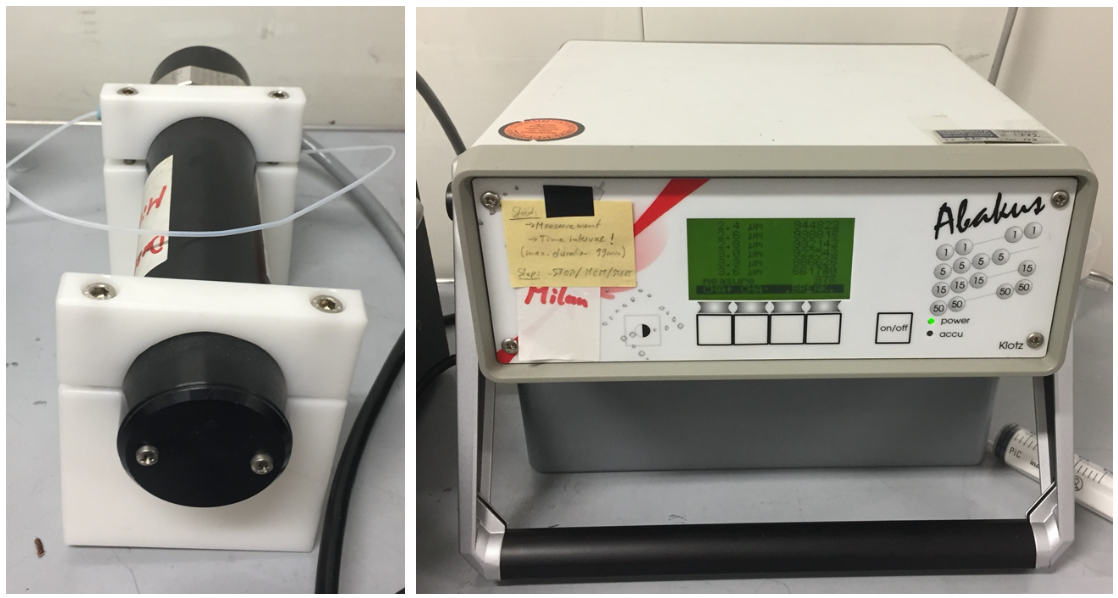
\includegraphics[scale=0.3]{abakus.png}
	\caption{The Abakus Laser Sensor (left) and its relative data processing Black Box (right).}
	\label{abakus_img}
\end{figure}
\newline
The instrument is made up by two parts, a detection cell and a case for data processing - as the output data visualized on the LCD screen are not the voltages recorded by the detector, but number of counts of particles with extinction diameter ($d_{ext}$) greater than a given value. To make an example, if the bin 2.4 $\mu$m reports $N$ counts, it means that $N$ particles with d$_{ext}$ $\geq$ 2.4 $\mu$m were counted during the run. \\
While operating, the sample is pumped in the cell \footnote{The diameter of the cell is typical for the sensor, so we will have to access it using a suitable pipe.}, where a laser beam ($\lambda =$ 670 nm) illuminates a photodiode sensor. Obviously, the presence of a particle would result in a negative peak in the transmitted power: this is counted in one of 32 possible bins (corresponding to 32 freely definable size classes), depending on its amplitude. This is why, if we want to produce a dimensional spectra, we absolutely need an accurate calibration (which is not straightforward, as the weight of the two contributions to extinction varies non-trivially depending on the dimensions of the particle). 

\subsection*{Technical Specifications} 
\begin{table}[!hp]
\centering
\renewcommand{\arraystretch}{1.2}
\begin{tabular}{l|l}
\hline
\hline
\textbf{Display and control} & background-lighted graphical LCD display, 6-key-operation \\
\textbf{Measuring mode} & single or continuous measurement with a cycle period of 1 – 99 min \\
\textbf{Data contents} & date, time, sample number, 32 freely programmable \\
& particle size channels \\
\textbf{Representation} & cumulative and distributive particle number, \\
& volume percent distribution, conversion in the standards USP 23, \\
& ISO 4406, NAS 1638 \\
\textbf{Alarm level} & for particle number, programmable for ISO or NAS classes \\
\textbf{Printer} & thermal printer DPU 414 \\
\textbf{Computer interface} & RS 232 C (V. 24) \\
\textbf{Power supply} & 230/115 VAC, 50/60 Hz, max. 10 W \\
\hline
\hline
\end{tabular}
\caption{Technical data and specification about the Abakus particle counter.}
\end{table}

\vspace*{1.0 cm}
Since at present there is no available official software from Klotz for data acquisition and for the subsequent analysis, an \textit{ad hoc} Python3.9 program has been written as described in the following sections.


%%%%%%%%%%%%%%%%%%%%%%%%%%%%%%%%%%%%%%%%%%%%%%%%%%%%%%%%%%%%%%%%%%%%%%%%%%%%%%%%%%%%
%%%%%%%%%%%%%%%%%%%%%%%%%%%%%%%%%%%%%%%%%%%%%%%%%%%%%%%%%%%%%%%%%%%%%%%%%%%%%%%%%%%%


\chapter{Graphical user interface (GUI)}
\label{gui_chpt}

In order to make the software user-friendly and easily accessible, a suitable GUI interface was built in parallel. 
Fig.(\ref{abakus_software}) shows what the starting interface looks like.
\begin{figure}[!hp]
	\centering
	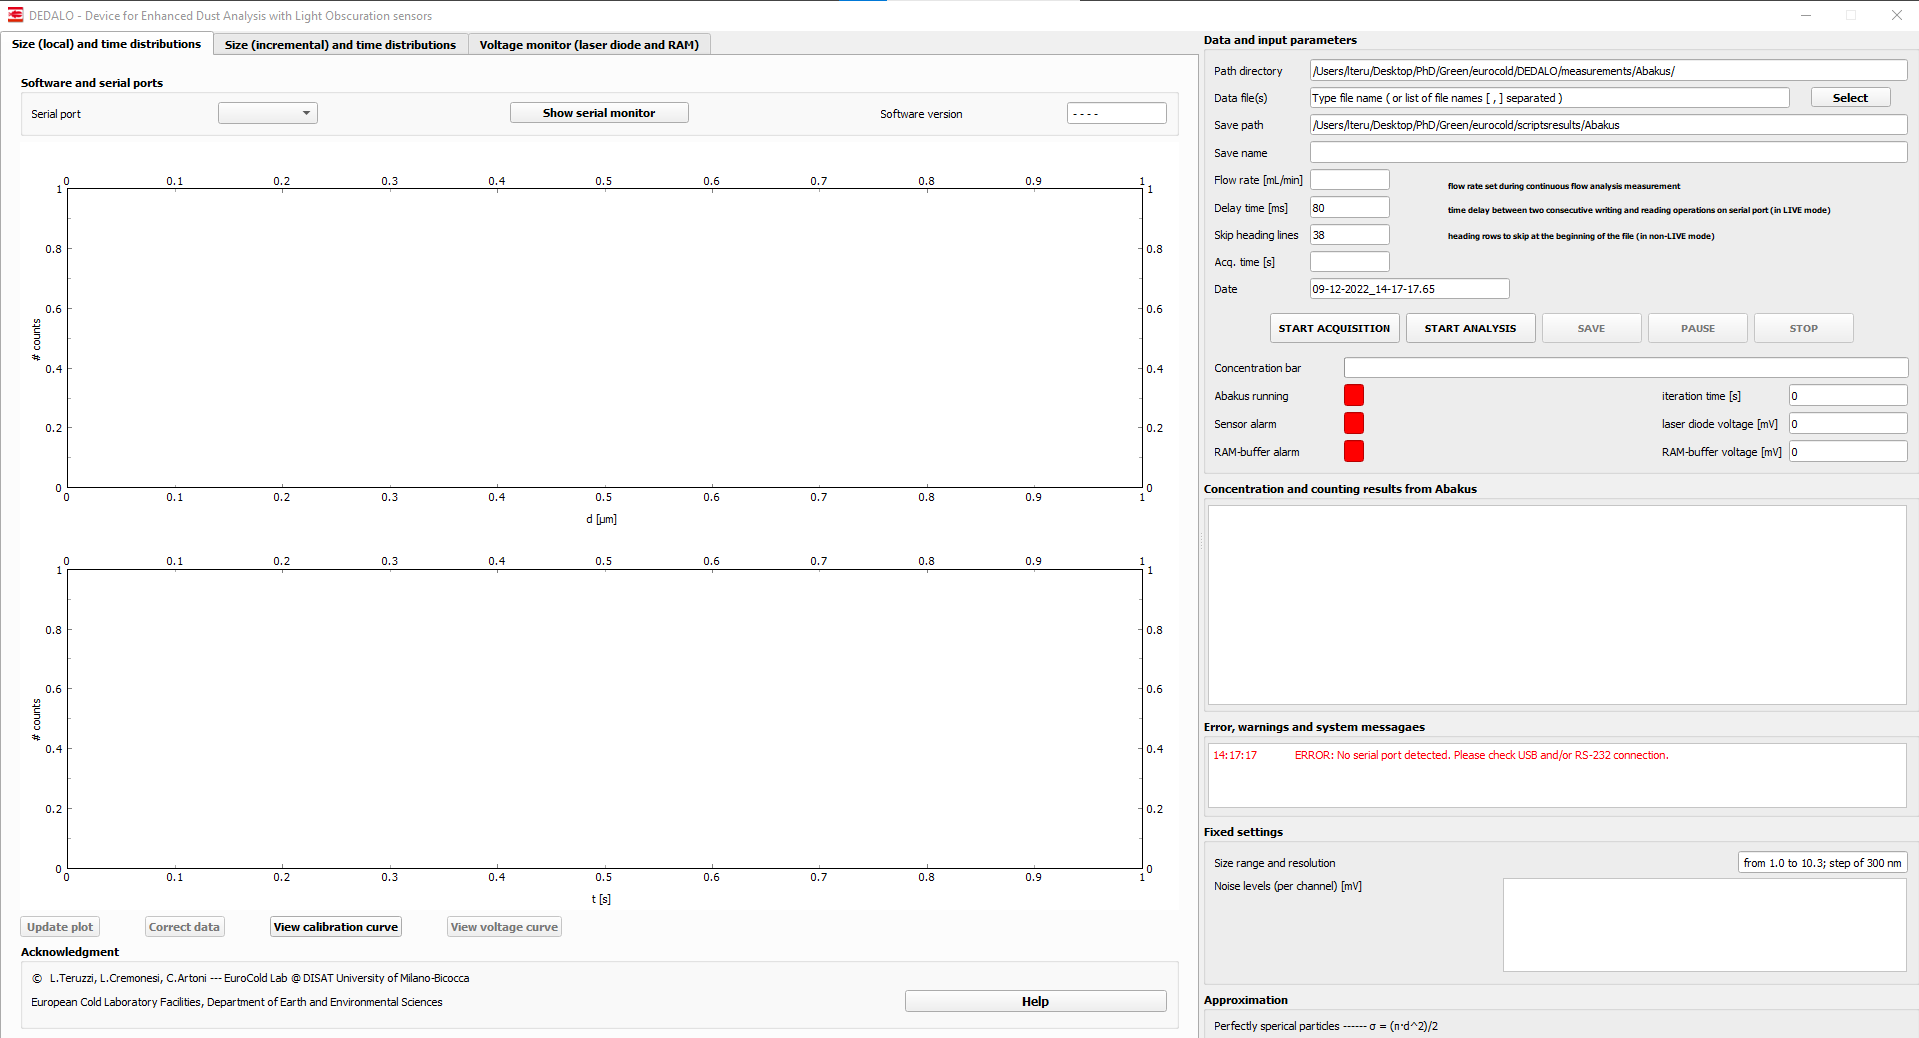
\includegraphics[scale=0.32]{abakus_software.png}
	\caption{GUI application, written in Python3.8 programming language, designed for Abakus laser sensor. Generally, the interface is divided in two halfes: on the left, some plots and histograms are shown while on the right the user can both specify the required input parameters and read the results from data analysis. Moreover, there is the possibility to perform some data analyses, investigating refractive index values different from the default one for Abakus sensor (n = 1.58), calibrate the instrument and visualize the noise level for each channel.}
	\label{abakus_software}
\end{figure}


%%%%%%%%%%%%%%%%%%%%%%%%%%%%%%%%%%%%%%%%%%%%%%%%%%%%%%%%%%%%%%%%%%%%%%%%%%%%%%%%%%%%
%%%%%%%%%%%%%%%%%%%%%%%%%%%%%%%%%%%%%%%%%%%%%%%%%%%%%%%%%%%%%%%%%%%%%%%%%%%%%%%%%%%%


\newpage
\section{Settings and default values}
\label{settings_sect}
In the following, each element in the right GUI interface is described.
\begin{figure}[!hp]
	\centering
	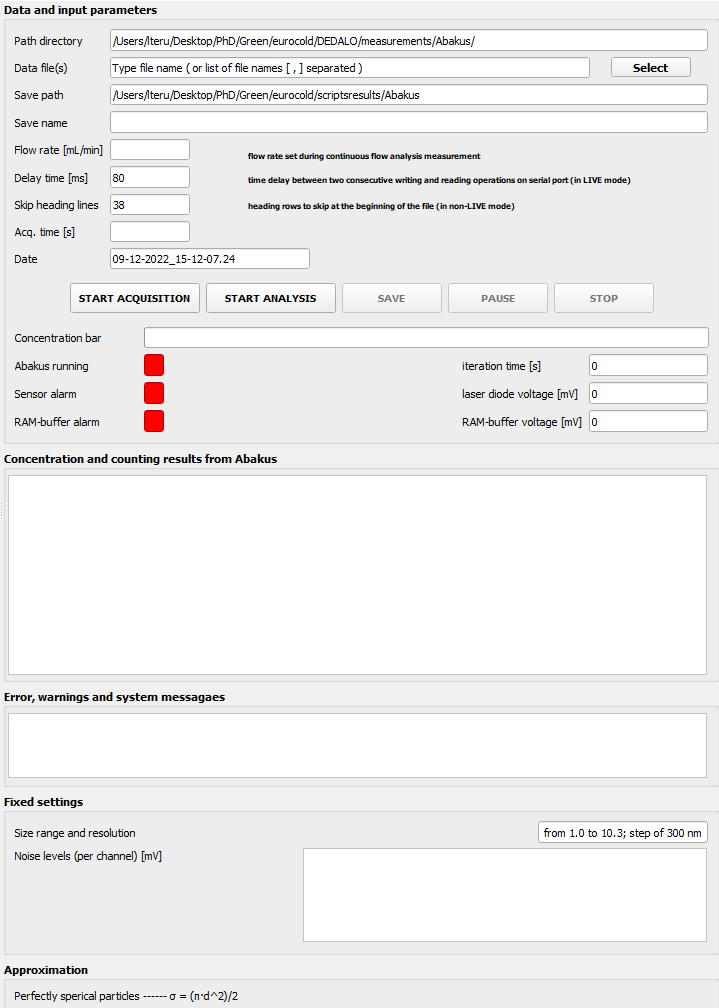
\includegraphics[scale=0.73]{setting_section.png}
	\caption{Example of the right side of thee GUI software, regarding all the settings and the parameters required to run correctly the measurement.}
	\label{setting_window}
\end{figure}
\begin{itemize}
\item \textbf{Data and input parameters}
\begin{itemize}
\item[-] \underline{Path directory}: path were the files (.txt, .dat) containing full data from Abakus laser sensor, as read via serial port RS-232, are stored.
\item[-] \underline{Data file(s)}: file(s) name the user wants to analyze; this input can consist of both a single name and a list of names, separated by a comma (" , ").
The histogram in the firts left panel is always referred to the first file specified in the list, while for a comparison of all the input files the user can switch to the third panel where their normalized \footnote{The aim of such a normalization is only to make the histograms correctly comparable at sight, dividing each column by the total number of countings.} histograms are shown.
\item[-] \underline{Save path}: path were the result files (.txt, .dat) are saved.
\item[-] \underline{Save name}: name specified by the user (WITH .txt or .dat extension) for saving.
\item[-] \underline{Flow rate}: measured in mL/min, it is the flow rate set on the peristaltic pump during the CFA measurement.
\item[-] \underline{Skip heading lines}: number of heading rows to skip before preforming the analysis. These lines consist of a series of information concerning the measurement previously performed with the Abakus laser sensor (Date and time of the acquisition, software version, noise levels and so on).
\item[-] \underline{Acquisition time}: measured in seconds, it is the specific period the user wants to analyze.
\item[-] \underline{Date}: date and time of the measurement, saved also in the heading lines of the file.
\item[-] \underline{Buttons}:
\begin{itemize}
\item START ACQUISITION: this button allows to swich between two different operating modes of the software: if "Live" is OFF, when the "Run" button is selected the GUI application reads all the input paramter previously defined and performs the analysis of a pre-recorded data file. On the contrary, if the "Live" button is ON the software performs a real time analysis during the continuous flow measurement. In the following image you can see the initial output stating which commands have been sent to the instrument and what it is doing.
\begin{figure}[!hp]
	\centering
	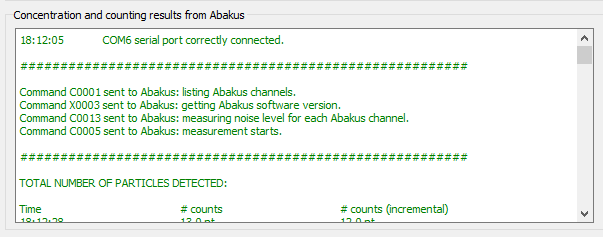
\includegraphics[scale=0.8]{measure_start.png}
\end{figure}
\item START ANALYSIS: this button starts the (serial reading and) analysis according to the option selected by "Live".
\item SAVE: this button allows the user to save all the results, also shown in the "Concentration and counting results from Abakus" output window, on a .txt file; the path to the correct directory and the file name are the ones specified before.
\item STOP: this button stops the measurement and disconnects the Abakus laser sensor.
\item PAUSE: this button stops temporarily the Abakus measurement; when pressed again, the measurement restarts.
\end{itemize}
\item [-] \underline{Concentration bar}: status bar which reports the sample particle concentration as a percentage of the maximum concentration detectable by the instrument.
\item[-] \underline{Abakus running}: check if the instrument in working properly by changing its color from red to green; if a problem of any kind is detected, the label becomes red again.
\begin{itemize}
\item iteration time: measured in milliseconds, it measures in real time the gap between two consecutive serial readings.
\end{itemize}
\item[-] \underline{Sensor alarm}: check if the laser voltage is being measured correctly by changing its color from red to green; if any problem is detected or if the regulating voltage exceeds 7000 mV, the label becomes red again.
\begin{itemize}
\item laser diode voltage: measured in mV, it is the regulation voltage of the laser diode inside the instrument; it is a very important parameter, since if the voltage exceeds 8000 mV, the sensor must be switched off immediately and cleaned up.
\end{itemize}
\item[-] \underline{RAM buffer alarm}: check if the RAM buffer voltage is being measured correctly by changing its color from red to green; if any problem is detected or if the voltage is lower than 2800 mV, the label becomes red again.
\begin{itemize}
\item RAM buffer voltage: measured in mV; as the laser diode regulating voltage, it is a very important parameter since if it becomes lower than 2800 mV, the sensor must be switched off immediately and cleaned up.
\end{itemize}
\end{itemize}
\item \textbf{Concentration and counting results from Abakus}: during a LIVE measurement, in this output window are visualized the number of particles detected by the sensor each second and the total incremental number pf counts since the beginning of the measurement. \\
On the other hand, if the software is running in non-LIVE operating mode, results are shown concerning the total number of particles detected by the Abakus, the total particle concentration and the partial concentrations for each channel as well.
\begin{figure}[!hp]
	\centering
	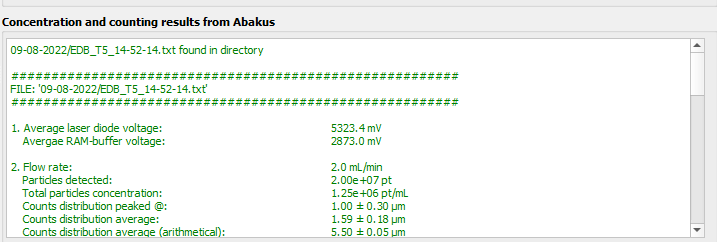
\includegraphics[scale=0.8]{analysis_start.png}
\end{figure}
\newpage
\item \textbf{Error, warnings and system messages}: in this output window are visualized warnings and/or error messages occurred during the software running. \\
\begin{figure}[!hp]
	\centering
	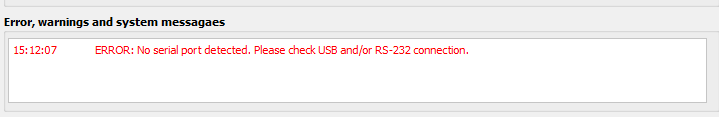
\includegraphics[scale=0.8]{error.png}
	\caption{Example of message (warning, specifically) reported in the error box. All the messages displayed here are printed in red. Here, the "Abakus running", the "Sensor alarm" and the `'RAM-buffer alarm'' labels are both red, since the software is not running yet.}
	\label{abakus_software3}
\end{figure}
\newline
\item \textbf{Fixed settings}
\begin{itemize}
\item[-] \underline{Software version}: kind of software originally supported by the Abakus laser sensor.
\item[-] \underline{Size range}: diameter range the instrument can measure, from 1.0 up to 10.3 $\mu$m.
\item[-] \underline{Resolution}: the difference in diameter that the Abakus laser sensor can resolve; in our case, it is equal to 300 nm.
\item[-] \underline{Noise levels (for each channel)}: noise levels measured by the Abakus laser sensor itself before the measurement starts.
\end{itemize}
\item \textbf{Approximation}: simply here is specified that the Abakus sensor work in spherical approximation; this allows to derive a straighforward relation between the extinction cross-section (which is the physical parameter properly measured by the Abakus laser sensor) and the extinction diameter of the equivalent sphere:
\begin{equation*}
\sigma_{ext} = \pi \cdot \left( \dfrac{d_{ext}}{2} \right)^{2}
\end{equation*}
\end{itemize}


%%%%%%%%%%%%%%%%%%%%%%%%%%%%%%%%%%%%%%%%%%%%%%%%%%%%%%%%%%%%%%%%%%%%%%%%%%%%%%%%%%%%
%%%%%%%%%%%%%%%%%%%%%%%%%%%%%%%%%%%%%%%%%%%%%%%%%%%%%%%%%%%%%%%%%%%%%%%%%%%%%%%%%%%%


\newpage
\section{Software measurement and analysis section}
\label{section_layout}

On the left GUI interface the user can firstly find four different sections that can be selected by the corresponding button on top:
\begin{itemize}
\item \textbf{Size (local) and time distribution}: the panel shows two kind of plots: in the upper part the particle size distribution (blue) and in the lower one the temporal evolution of the number of counts (red line - yellow filling).
If the "Live" button is pressed, both the size distribution histogram and the time evolution plot are automatically update from time to time each second: the former shows the instant number of counts detected and the latter one is incremented consequently.
On the other hand, if the "Live" button is off, the time plot shows the entire temporal evolution during the measurement and by clicking on it the upper size distribution is updated to the number of particles detected at that instant. \\
\begin{figure}[!hp]
	\centering
	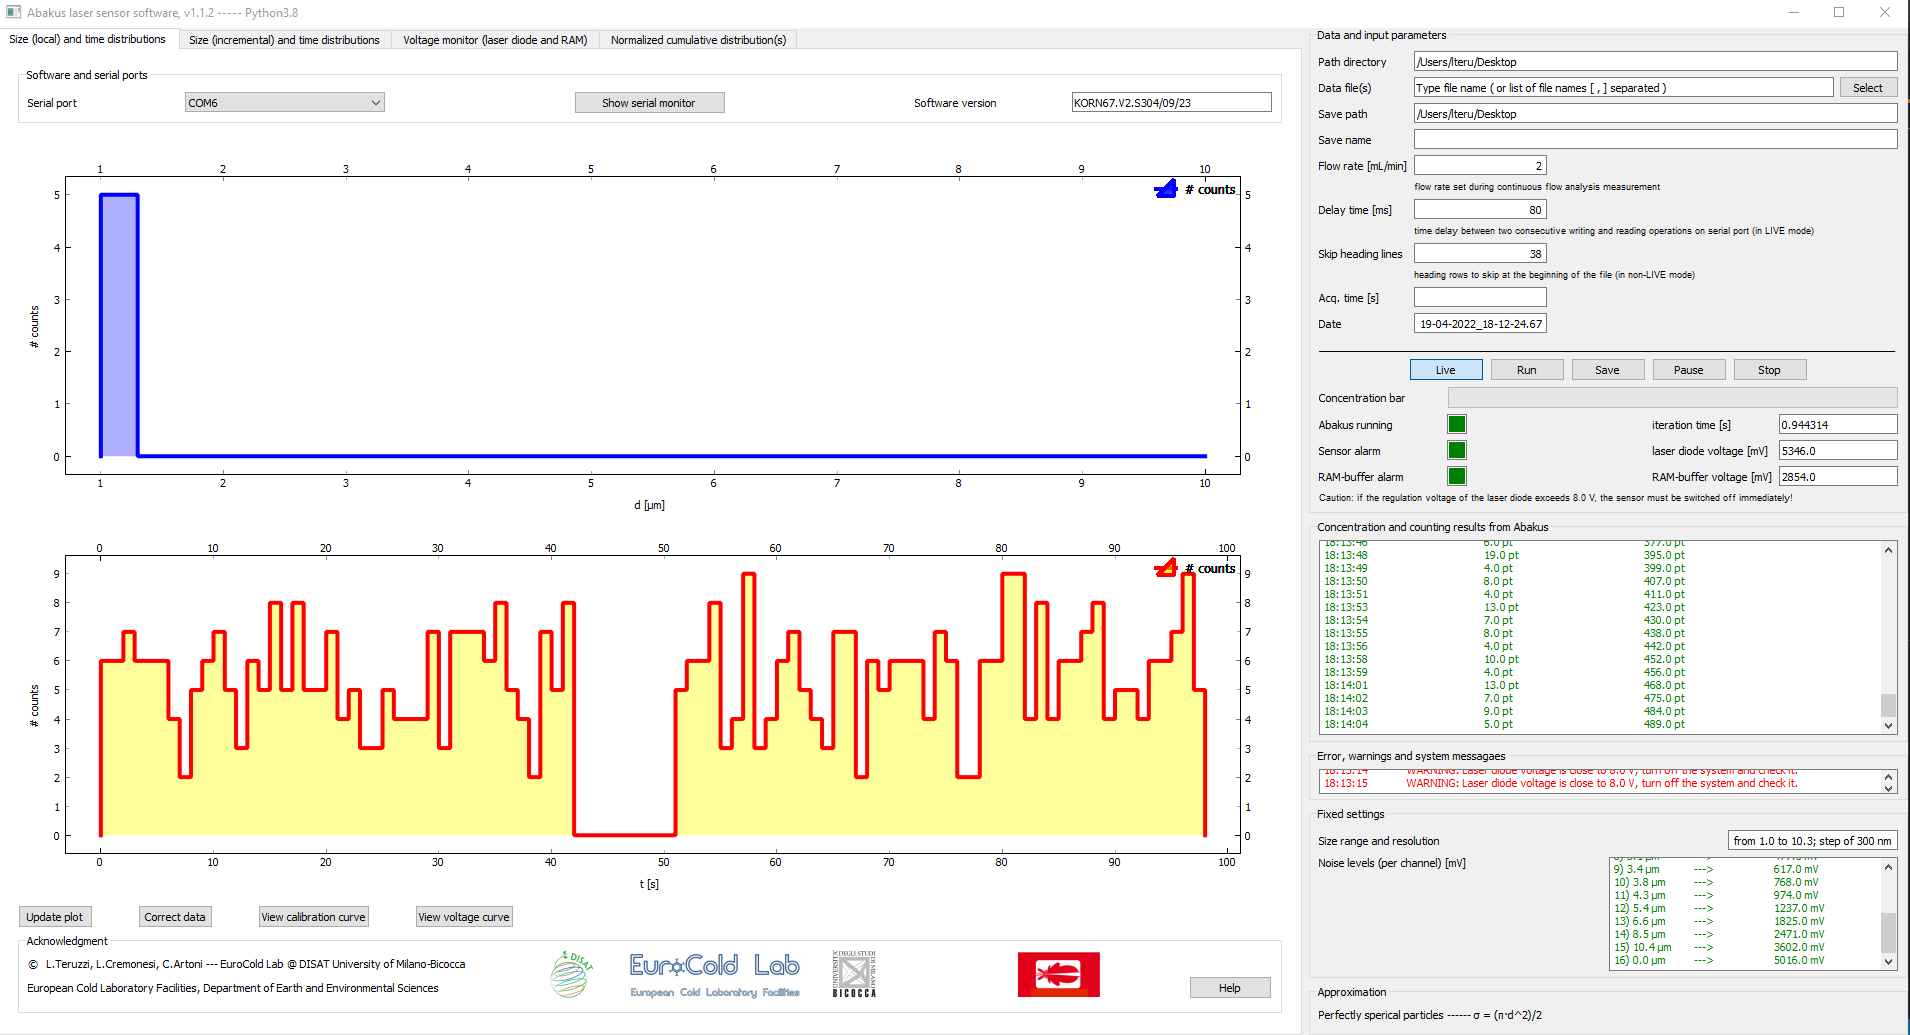
\includegraphics[scale=0.3]{local_measure.png}	
	\caption{Example of the 'Size (local) and time distribution' section. On the left side of the GUI interface, the particle size distribution (blue) and the temporal evolution of the number of counts (red line - yellow filling); the first one represents the number of counts as a function of the particle diameters [$\mu$m] as set by the user in the 32 Abakus channels, while in the latter they are visualized as a function of time [s]. On the right side, in the central output window the user can see for each acquisition the number of particles detected (central column) and the total number of counts since the beginning of the measure (right column). The error output window reports with a red font any warning messages arising during the software operation and for the sake of completeness the ''Noise level window'' reports the voltage values [mV] of the instrument measuring channels.}
	\label{abakus_software1}
\end{figure}

\item \textbf{Size (incremental) and time distribution}: as for the previous one, this panel shows two kind of plots: in the upper part the incremental particle size distribution (blue) and in the lower one the temporal evolution of the number of counts (red line - yellow filling).
If the "Live" button is pressed, both the size distribution histogram and the time evolution plot are automatically update from time to time each second: the former shows the incremental number of counts detected by the instrument and the latter one is incremented consequently.
On the other hand, if the "Live" button is off, the time plot shows the entire temporal evolution during the measurement and by clicking on it the upper size distribution is updated to the total number of particles detected until then (note: not the instant number of counts but the incremental one!). \\
\begin{figure}[!hp]
	\centering
	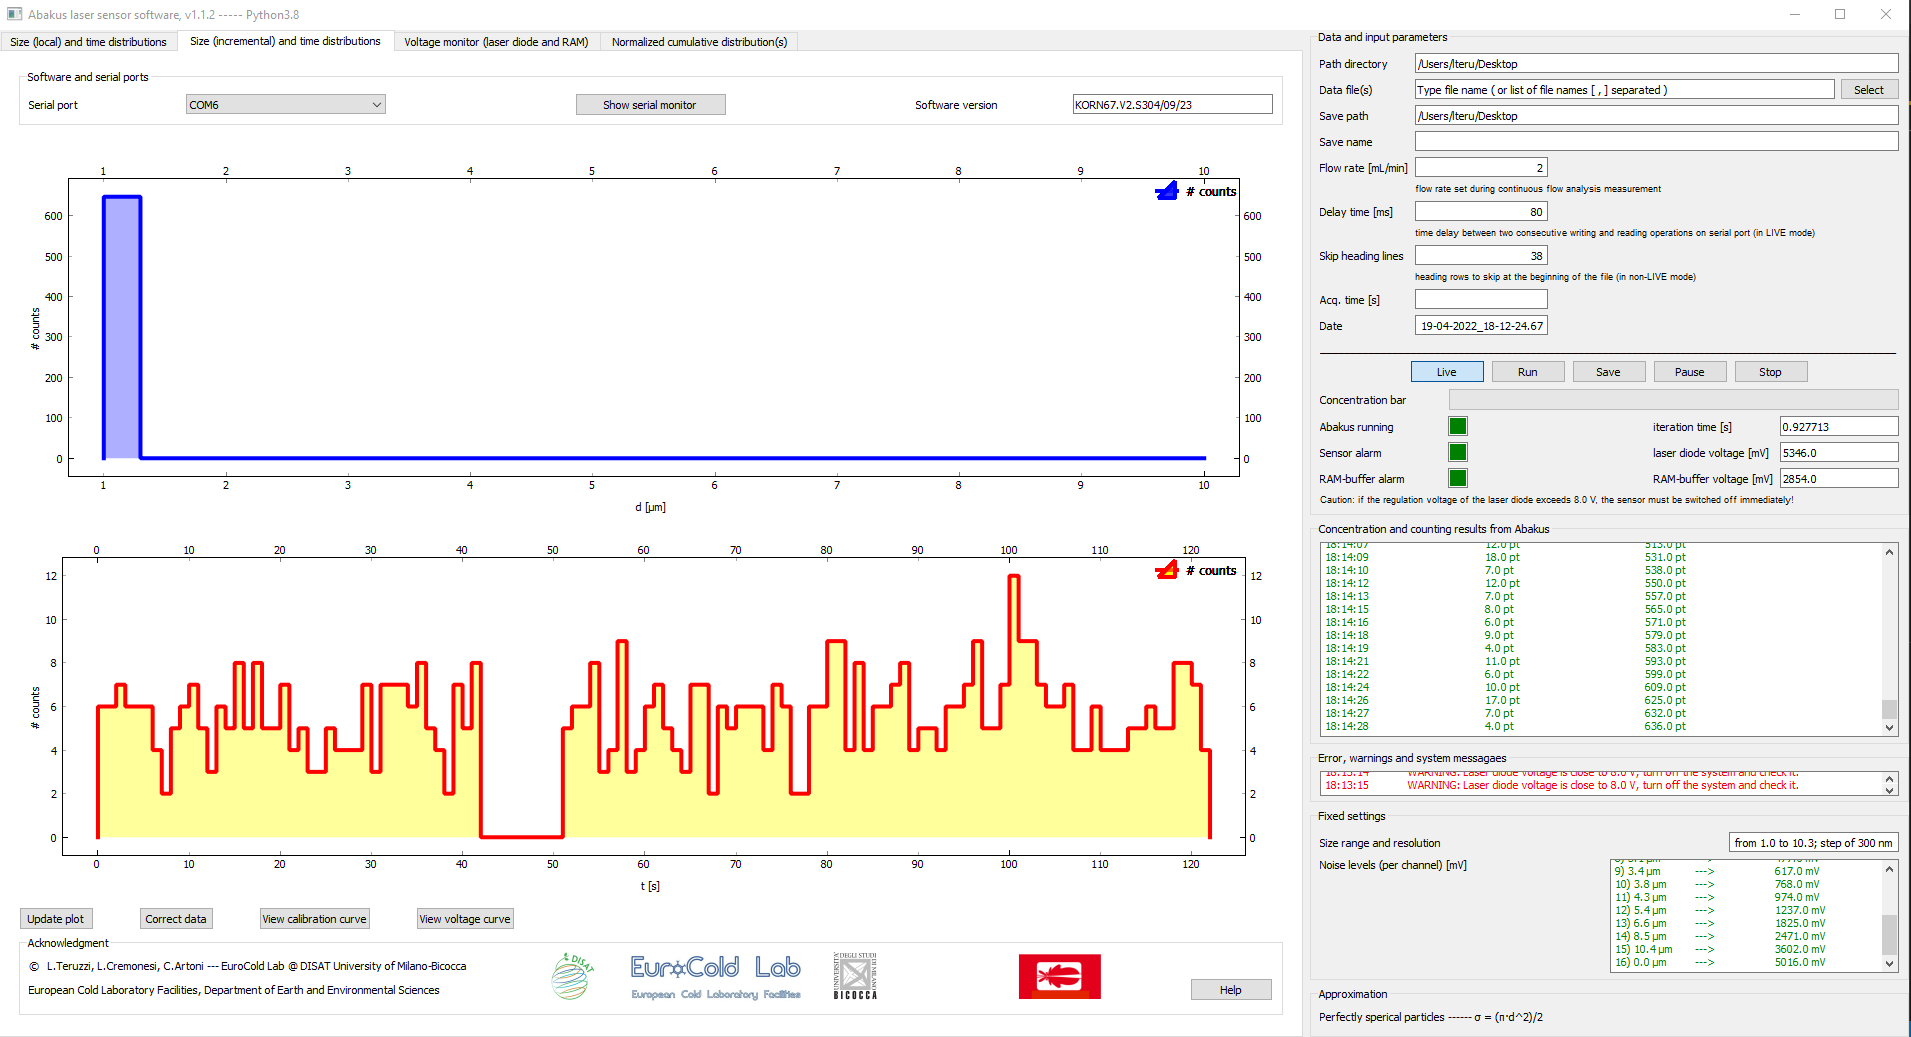
\includegraphics[scale=0.3]{incremental_measure.png}
	\caption{Example of the 'Size (incremental) and time distribution' section. On the left side of the GUI interface, the particle size distribution (blue) and the temporal evolution of the number of counts (red line - yellow filling); the first one represents the number of counts as a function of the particle diameters [$\mu$m] as set by the user in the 32 Abakus channels, while in the latter they are visualized as a function of time [s]. Unlike the previous situation, here the size distribution shows the incremental number of counts for each channel and not the instant measurement. On the right side, the software settings and properties of the output windows are the same as described above (see Fig.\ref{abakus_software1}).}
	\label{abakus_software2}
\end{figure}

\item \textbf{Voltage monitor (laser diode and RAM)}: the panel shows the behavior of both the laser (red line) and the RAM-buffer voltages (blue line) throughout the measurement. As stated previously, the laser supply voltage should stay below 8000 mV and the RAM-buffer one should be not lower than 2800 mV. \footnote{Sometimes it happens that for just one second the former or the latter voltage value "explodes" (that is, it becomes very large) and during the next acquisition it gets back to the default value: don't worry, it may be some kind of serial communication error and a red warning message should be visualized in the corresponding box. If the over-voltage persists, that is a problem.}
\begin{figure}[!hp]
	\centering
	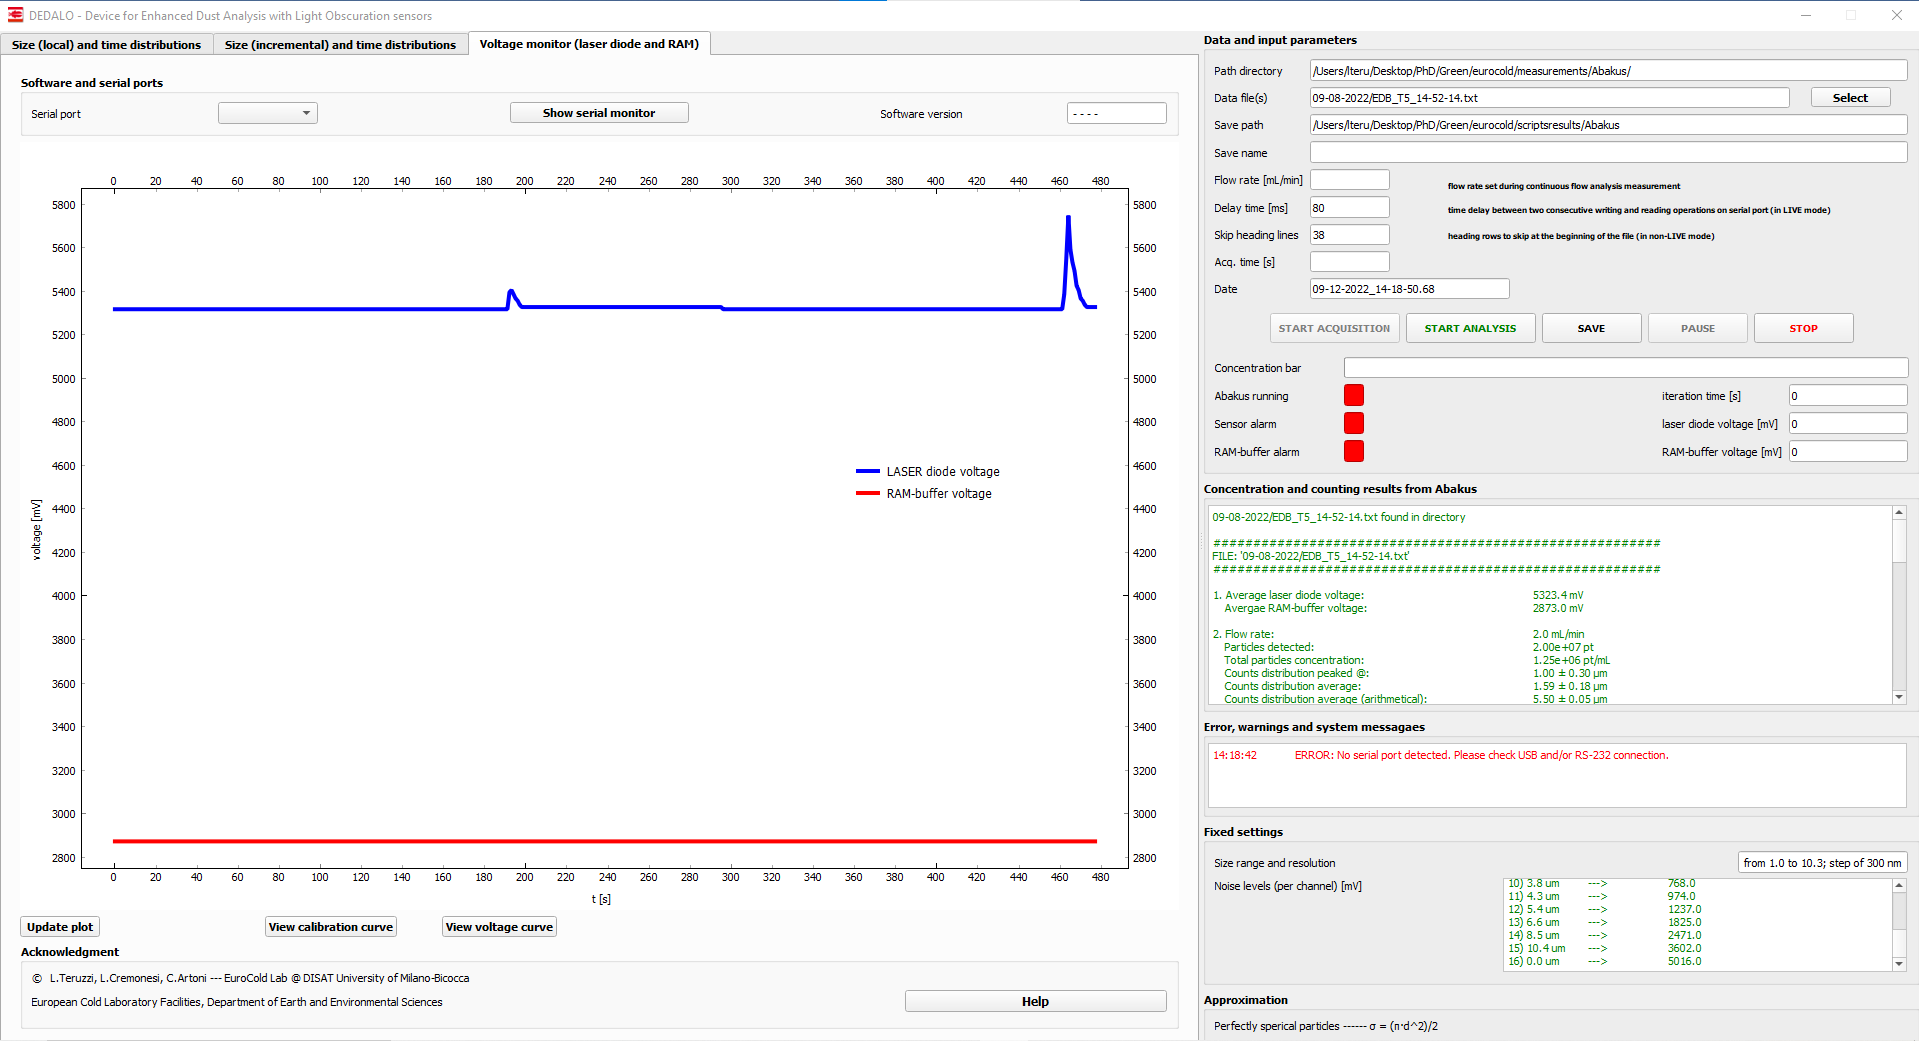
\includegraphics[scale=0.3]{voltage_measure.png}
	\caption{Example of the 'Voltage monitor (laser diode and RAM)' section. On the left side, during a "Live" acquisition the user can see in real time the behavior of the laser diode supply voltage (blue line) and the RAM-buffer voltage (red line). In standard operative conditions, the former should be about 5300 mV while the latter around 2800 mV. If the laser diode voltage exceeds 8 V (8000 mV) or the RAM-buffer voltage gets too low an error message raises and the user should switch the Abakus laser sensor off. NOTE: this picture shows clearly what is not supposed to happen to the laser diode voltage!}
	\label{abakus_software2}
\end{figure}
\end{itemize}

\newpage
Apart from the graphic rendering, some further and useful options are available. Starting from the top:
\begin{itemize}
\item \underline{Serial monitor}: this button opens a serial terminal in order to monitor the serial communication between the user laptop/PC and the instrument. By default, when opened this monitor acts as an output monitor: when the measurement is running, each second the Abakus serial answer is visualized as a Python bytestring.
At the same time, if needed the user can also send serial command (according to the instrument protocol) and check the corresponding output.
\item \underline{Update plot}: the user can choose to select only a portion of the size distribution and the current plot (Size (local) and time distribution or Size (incremental) and time distribution) is updated consequently. The selected section is highlighted with a different color (red) and some statistical information on the distribution itself are visualized on a separate window: among them, for example, mean and median values, the diameter corresponding to the peak of the size distribution.
This button can be pressed multiple times and the plot is always updated to the last desired portion.
\item \underline{Correct data}: the user can press this button if it is required to perform some deeper analyses on the size distribution directly measured by the Abakus particle counter, such as correction with the appropriate calibration curve or the fit with different refractive indices values. These procedures are better described in the following section.
\item \underline{View calibration curve}: the instrumental calibration curve is visualized. This curve was retrieved by measuring some well known and calibrated samples, composed of colloidal suspensions of polystyrene spheres with fixed diameters \footnote{The polystyrene samples available in the laboratory were 1.0, 1.5, 2.1, 2.9, 3.78, 5.0 and 5.45 $\mu$m in diameter.}, and checking their deviation from the Mie scattering theory prevision. As stated above, the definition of this calibration function and its importance are better presented in the following. \\
This button can be pressed both in "Live" and in non "Live" operating mode.
\item \underline{View voltage curve}: the 32 Abakus channel voltages are visualized, no more and no less. This button can be pressed both in "Live" and in non "Live" operating mode.
\item \underline{Help}: simply, this PDF manual is visualized.
\end{itemize}


%%%%%%%%%%%%%%%%%%%%%%%%%%%%%%%%%%%%%%%%%%%%%%%%%%%%%%%%%%%%%%%%%%%%%%%%%%%%%%%%%%%%
%%%%%%%%%%%%%%%%%%%%%%%%%%%%%%%%%%%%%%%%%%%%%%%%%%%%%%%%%%%%%%%%%%%%%%%%%%%%%%%%%%%%


\newpage
\section{Data analysis}
\label{analysis_sect}

By clicking the "Correct data" button, a small interactive window is visualized so that the user can select which kind of analysis to perform, as represented in Fig.(\ref{correct_data}). Three main options are available, even though only two of them ($\#$1 and $\#$2) are well implemented and currently working and are presented in the following.

\begin{figure}[!htb]
	\centering	
	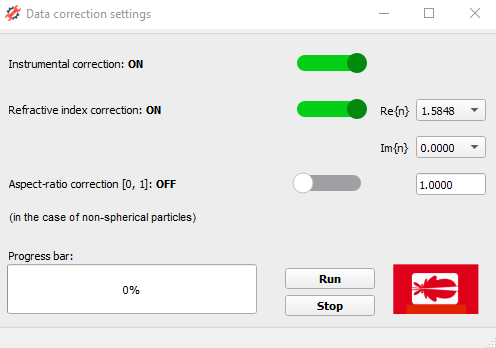
\includegraphics[scale=0.75]{correct_data.png}
	\caption{Data correction window. Three possible solutions for correcting and calibrating Abakus measurements are reported: (1) calibration with known calibrated samples (colloidal suspension of polystyrene nanoparticles) and comparison to Mie scattering theory; (2) refractive index correction, which is of fundamental importance in order to increase Abakus measurements accuracy; (3) aspect-ratio correction, in the case of non-spherical particles.}
	\label{correct_data}
\end{figure}
After the ''Run'' button is pressed, the progress bar reports the computation and analysis status.
\begin{figure}[!htb]
	\centering	
	
\includegraphics[scale=0.75]{correct_data1.png}
\end{figure}

\subsection{User calibration from extinction measurements}
\label{ext_calibration_subsection}

This data correction is purely of instrumental kind. The problem is that the Abakus channel voltages probably are not the correct ones to optimally perform the measurements, retrieving the particle size distribution. \footnote{NOTE: this problem refers only to THIS instrument in the EuroCold Lab of the University of Milano Bicocca, it might not show up in other devices.}
Thus, a calibration is needed to match the output of the Abakus laser sensor with the correct values. 
This kind of calibration was performed as described below. 
\begin{itemize}
\item Some samples were prepared consisting of a colloidal suspension of polystyrene calibrated nanoparticles with refractive index of about 1.58 at 670 nm wavelength. The choice of such a sample is motivated by the fact that the instrument measures the size distribution as if the particles contained in the sample all had refractive index value of 1.58 (that's exactly what motivates, by the way, the upcoming correction in \ref{RI_calibration_subsection}). 
The colloidal suspensions were characterized by different particle diameters, nominally 1.0, 1.5, 2.1, 2.9, 3.78, 5.0 and 5.45 $\mu$m.
\item As a further confirmation, the particle diameters were independently measured by means of a Coulter Counter (Multisizer 4 particle analyser, Beckman Coulter \cite{CC}) as well.
\item After performing the measurement with the Abakus laser sensor, the results were compared with the theoretical value from Mie scattering theory (some notes on Mie theory are provided in Appendix A). 
It was found that there was a (small but appreciable) deviation for the expected values, thus making it necessary to compensate it.
\item The instrumental calibration was defined as the function such that the measured diameter divided by the calibration function corresponds exactly to the extinction diameter. In order to do so, the ratio between the measured values and the theoretical ones was computed and these data were fitted with a polynomial function (to avoid artifacts in the calibrated distribution, the calibration function has to be a continuous function of the measured diameter with a continuous first derivative).
\end{itemize}
In Fig.(\ref{calibration_plot}) are reported the comparison between the measured diameters and the Mie extinction curve \footnote{Note that the extinction diameter was retrieved from the extinction cross section under spherical approximation} (Fig.(\ref{calibration_plot}a)) and the calibration function  (Fig.(\ref{calibration_plot}b)).

\begin{figure}[!htb]
	\captionsetup[subfigure]{labelformat=empty}
	\begin{subfigure}{.5\textwidth}
	\centering
	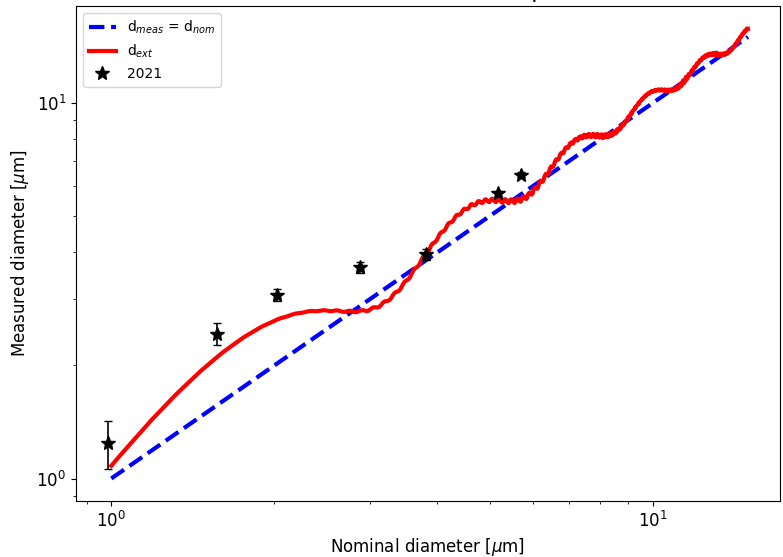
\includegraphics[scale=0.41]{abakus_calibration_1.png}
	\caption{(a)}
	\end{subfigure} 
	\begin{subfigure}{.5\textwidth}
	\centering	
	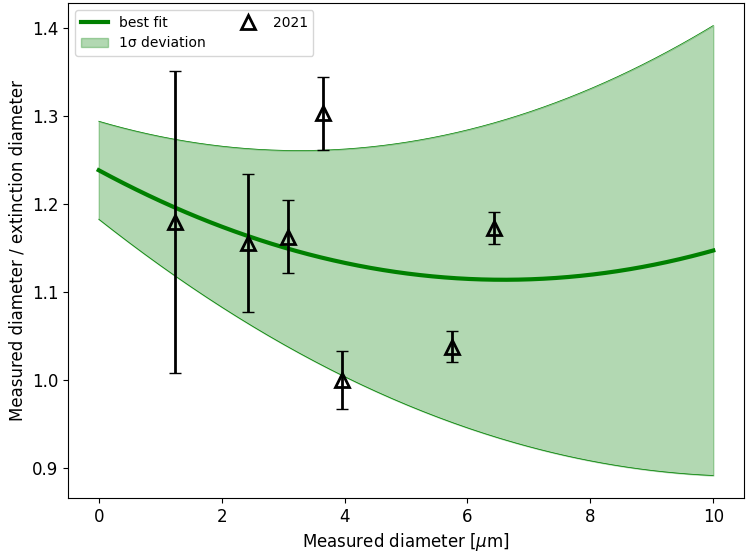
\includegraphics[scale=0.42]{abakus_calibration_2.png}
	\caption{(b)}
	\end{subfigure} 
	\caption{Abakus calibration function. (a) Comparison between the measured extinction diameters of colloidal suspensions of polystyrene nanoparticles (refractive index about 1.58, variable sizes) and the extinction curve derived from Mie scattering theory. (b) Calibration function obtained by fitting the diameter ratios to a polynomial function.}
	\label{calibration_plot}
\end{figure}


\subsection{Refractive index correction}
\label{RI_calibration_subsection}

The correction described in this section arises from the fact that the instrument’s manufacturing calibration is based on (spherical) particles with fixed refractive index of 1.58, thus leading to alterations and uncertainties in the measured size distribution. 
Moreover, the discrepancy gets larger and larger with increasing refractive index values of the sample. \\
The main aim of this procedure is to develop a reliable and consistent method to overcome this limitation and make it possible to measure particle size distributions on the basis of a more suitable refractive index depending on the effective sample composition. This will increase the accuracy of Abakus measurements and improve future ice core record comprehension and intercomparisons.
As a starting point, some look-up tables (LUT) were computed through Mie scattering theory for perfectly spherical, smooth and homogeneous particles varying the particle diameter form 0.2 $\mu$m to 20 $\mu$m and the relative refractive index of the sample with respect to the surrounding medium (in our case, water with n$_{H2O}$ = 1.3310) from 1.00 to 1.98 approximately.
In doing so, not only real refractive index values were considered but also the case of (low) absorption, so the sample refractive index was characterized by an imaginary part as well.
In Fig.(\ref{cext_2D}) is shown an example of such bidimensional LUT (on the left) and a 1D profile extracted from the former.
\begin{figure}[!htb]
	\centering	
	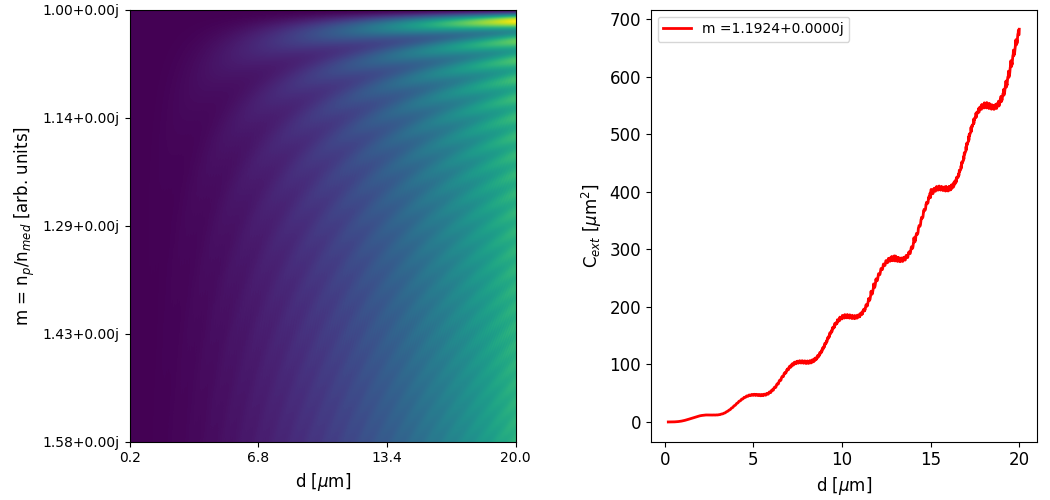
\includegraphics[scale=0.6]{Cext_2D.png}
	\caption{Trend of C$_{ext}$ for an aqueous suspension spherical particles with different refractive indices, as a function of particles diameter between 0.1 and 10 $\mu$m.}
	\label{cext_2D}
\end{figure}
\newline
The correction over the refractive index works as follows:
\begin{itemize}
\item The algorithm takes as input parameter a list of the Abakus measurable diameters (eg. the diameter values set by the user on each one of the 32 programmable instrument channels or the calibrated ones, if the instrumental calibration is performed first). From the LUT in Fig.(\ref{cext_2D}) the 1D profile relative to n$_{p}$ = 1.5848 is retrieved and for each measured diameter the corresponding optical extinction cross section is found.
\item Depending on the value specified by the user in the correction window, a second 1D curve is selected from the LUT and from this is calculated the value of d such that the extinction cross section is equal to that calculated in the previous point.
Here is a limitation of this method: as you can see, when it comes to determine the particle diameter from the extinction cross section it is not so easy, since the function is not reversible and a single value of C$_{ext}$ may correspond to multiple diameters; in addition, there are some regions where the extinction cross section fluctuates around an almost constant value for multiple possible diameters: obviously,this can be reflected in strong uncertainties in the particle size reconstruction.
To overcome this problem, the simplest solution that can be adopted is to fit the Mie extinction curve to a polynomial function (which is, as stated before, a continuous function with a continuous first derivative) to which refer for the procedure just described. However, this solution is effective for small values of the relative refractive index but gradually fails (that is, the agreement between the two curves decreases) for larger values. Because of this, in further versions of this software other possibilities will be examined to maximize the algorithm reliability.
\item The new diameters retrieved after this procedure allow to rescale the particle size distribution as measured by the Abakus laser sensor accounting for a refractive index value different from the default one.
\end{itemize}


\subsection{Aspect-ratio correction}
\label{AR_calibration_subsection}

This is the case of non-spherical particles (such as prolate or oblate spheroids, plates or disks), but is STILL WORK IN PROGRESS... \\
It will be of fundamental importance to implement also this kind of correction since the Abakus laser sensor relies on the spherical particles approximation, resulting in obvious alternations of the real particle size distribution of the sample (since mineral dust particles are never spherical in shape).

\newpage

The analyses described in \ref{ext_calibration_subsection}, \ref{RI_calibration_subsection} and \ref{AR_calibration_subsection} are organized in a single interactive window according to the following layout:
\begin{figure}[!htb]
	\centering	
	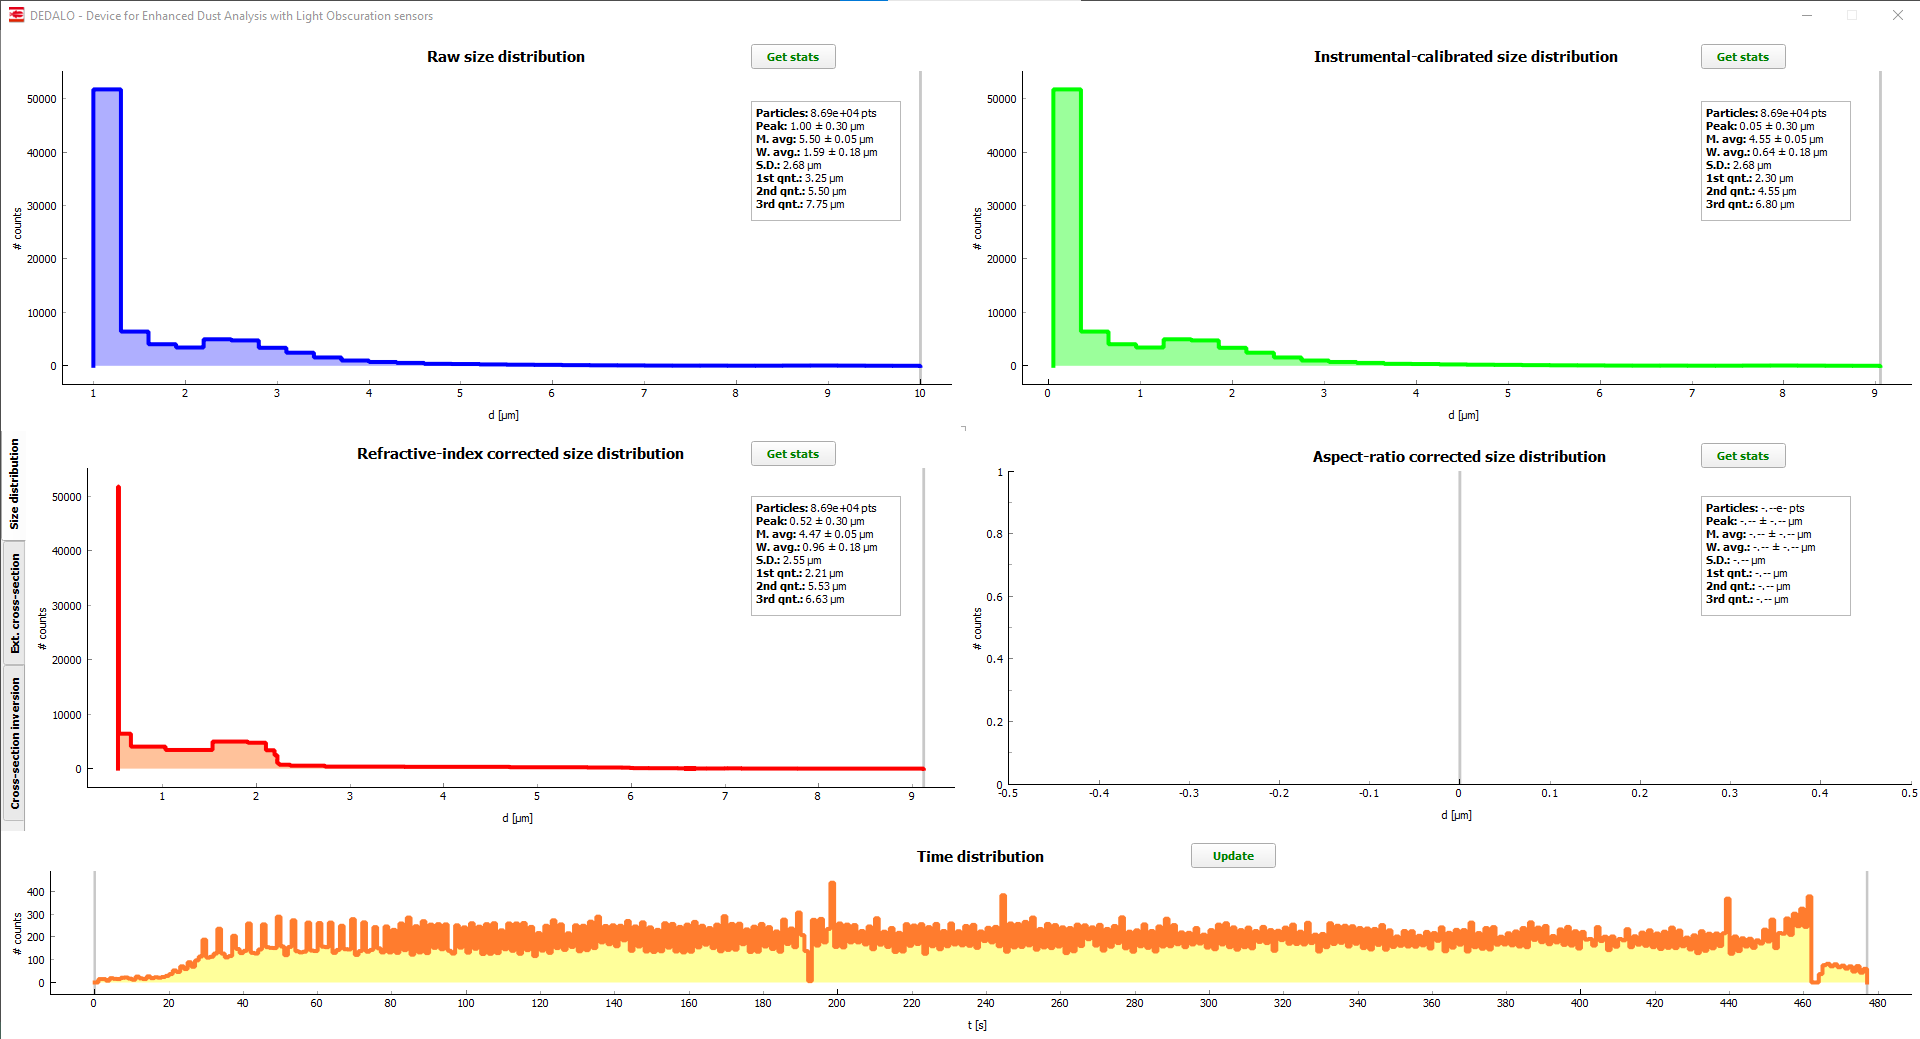
\includegraphics[scale=0.32]{plot_correction_1.png}
	\caption{Window resuming the different kind of analyses described above. The blue histogram in the upper left corner is the raw uncalibrated size distribution measured by the Abakus laser sensor; the green one, on the right, describes the calibrated size distribution starting from the considerations explained in Section \ref{ext_calibration_subsection}. Finally, the red size distribution in the lower left corner is the one obtained after the inversion with the refractive index value(s) set by the user in the appropriate window. Further information on this third procedure are presented in the following. On the bottom, the time distribution of the number of counts is reported as well, so that the user can choose to consider the whole measurement or just a slice of it (limiting consequently the number of particles visualized in the size distributions) by moving the vertical cursors.}
	\label{plot_correction}
\end{figure}
\newline
In the upper left corner the size distribution is the uncorrected raw one, as measured by the Abakus laser sensor, while on the right side the user can see the calibrated distribution (based on polystyrene extinction measurements). In the lower left corner it is visualized the size distribution after the compensation on the desired refractive index; lastly, the lower right corner is devoted to the aspect-ratio correction which is still work in progress. \\ \\
The section devoted to the refractive index inversion, as you can see, consists of three separate plots: the first one, immediately displayed when running the software, is precisely the size distribution after this kind of correction; the second one shows a comparison between the extinction cross-section curve for polystyrene perfectly smooth spheres @ 670 nm and the same function evaluated from Mie scattering theory for spherical particles of the selected refractive index.
Lastly, the third figure represents the inversion curve used for retrieving the corrected size distribution, that is the  particle diameter as a function of the extinction cross-section (red line), and the polynomial fit applied (black line).
\newpage

\begin{figure}[!htb]
	\captionsetup[subfigure]{labelformat=empty}
	\begin{subfigure}{1.\textwidth}
	\centering
	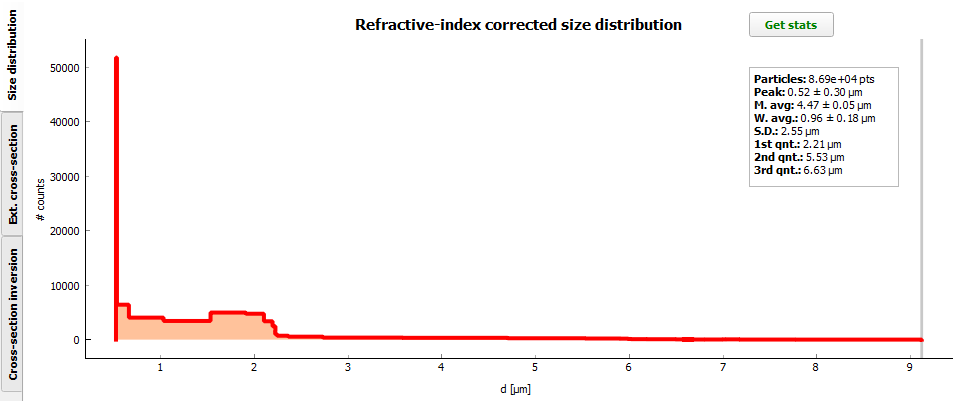
\includegraphics[scale=0.55]{plot_correction_2.png} 
	\caption{(a)}
	\end{subfigure} 
	\begin{subfigure}{1.\textwidth}
	\centering	
	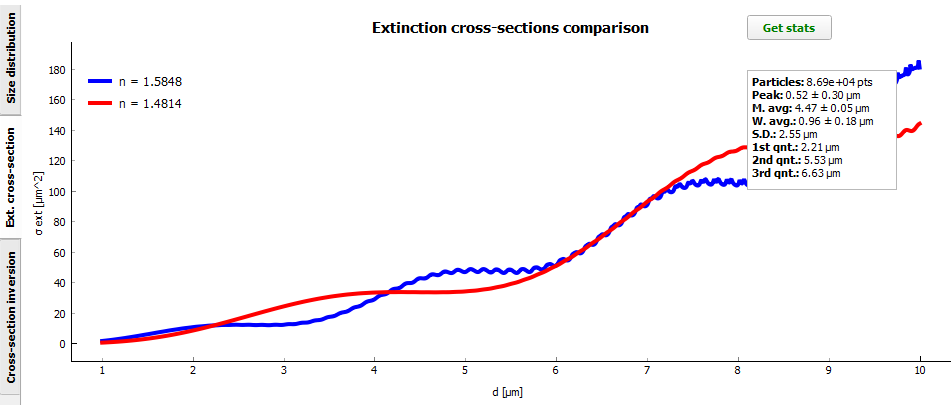
\includegraphics[scale=0.55]{plot_correction_3.png} 
	\caption{(b)}
	\end{subfigure} 
	\par\bigskip
	\begin{subfigure}{1.\textwidth}
	\centering
	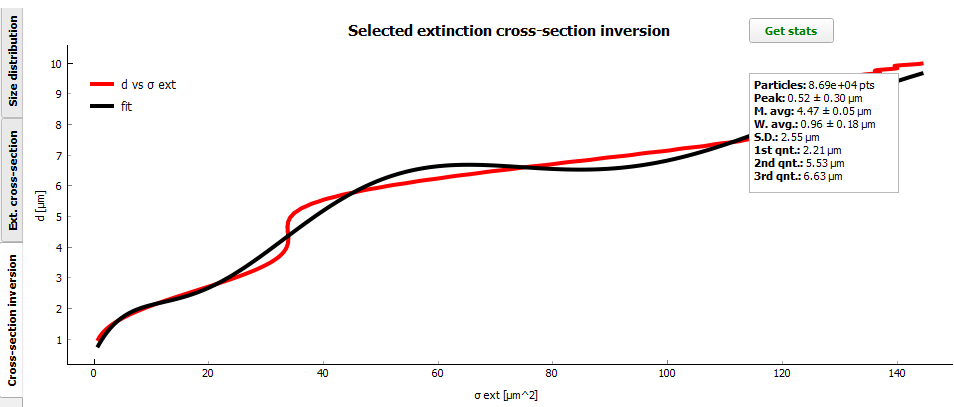
\includegraphics[scale=0.55]{plot_correction_4.png} 
	\caption{(c)}
	\end{subfigure} 
	\caption{.}
\end{figure}


%%%%%%%%%%%%%%%%%%%%%%%%%%%%%%%%%%%%%%%%%%%%%%%%%%%%%%%%%%%%%%%%%%%%%%%%%%%%%%%%%%%%
%%%%%%%%%%%%%%%%%%%%%%%%%%%%%%%%%%%%%%%%%%%%%%%%%%%%%%%%%%%%%%%%%%%%%%%%%%%%%%%%%%%%


\newpage
For more informations on the classes, funtions and methods used to achieve this software, plase have a look at Appendix B. \\
If you still have some doubts, questions or suggestions for making the software better and nicer, feel free to contact Luca Teruzzi: \\
\begin{itemize}
\item Phone number: +39 334 9801058
\item Mail: luca.teruzzi@unimib.it \\
                \hspace*{0.95 cm} luca.teruzzi@unimi.it
\end{itemize}


%%%%%%%%%%%%%%%%%%%%%%%%%%%%%%%%%%%%%%%%%%%%%%%%%%%%%%%%%%%%%%%%%%%%%%%%%%%%%%%%%%%%
%%%%%%%%%%%%%%%%%%%%%%%%%%%%%%%%%%%%%%%%%%%%%%%%%%%%%%%%%%%%%%%%%%%%%%%%%%%%%%%%%%%%


\newpage
\chapter{Appendix A: Mie theory and light extinction}

When a particle is illuminated by a beam of monochromatic radiation, the angular distribution of the scattered light depends strongly on the nature of the particle itself, i.e., its shape and size and the material of which it is composed. \\
In the following, the Mie scattering problem is addressed in the specific case of particles with spherical geometry, for which there is an exact analytical solution to the scattering problem.

The spherical wave scattered by the particle is modulated by the so-called scattering complement amplitudes $S_1(\theta)$ and $S_2(\theta)$, relative to the two different possible polarizations of the incident wave. They are analytically defined by the expressionsi \cite{BH, scattering_sphere_1}

\begin{equation}
	\vspace*{0.1 cm}
	\begin{cases}
	S_{1} \left( \theta \right) &= \sum\limits_{n=1}^{+\infty} \dfrac{2n+1}{n\left( n+1 \right)} \left[ a_{n}\pi_{n}\left( \cos\theta \right) + b_{n}\tau_{n}\left( \cos\theta \right) \right] , \\[10 pt]
	S_{2} \left( \theta \right) &= \sum\limits_{n=1}^{+\infty} \dfrac{2n+1}{n\left( n+1 \right)} \left[ b_{n}\pi_{n}\left( \cos\theta \right) + a_{n}\tau_{n}\left( \cos\theta \right) \right] , 
	\end{cases}
	\vspace*{0.2 cm}
	\label{S12_sphere}
\end{equation}

\noindent dove $\theta$ rappresenta l'angolo di scattering.

The scattering coefficients $a_n$ and $b_n$ that determine the behavior of the spherical wave scattered by the particle are given by the following relations \cite{BH, VdH}:
\begin{equation}
	\vspace*{0.1 cm}
	\begin{cases}
	a_{n} = \dfrac{m \psi_{n} \left( mx \right) \psi_{n}^{'}\left( x \right) - \psi_{n} \left( x \right) \psi_{n}^{'}\left( mx \right)}{m \psi_{n} \left( mx \right) \xi_{n}^{'}\left( x \right) - \xi_{n} \left( x \right) \psi_{n}^{'}\left( mx \right)} , \\[10 pt]
	b_{n} = \dfrac{\psi_{n} \left( mx \right) \psi_{n}^{'}\left( x \right) - m\psi_{n} \left( x \right) \psi_{n}^{'}\left( mx \right)}{\psi_{n} \left( mx \right) \xi_{n}^{'}\left( x \right) - m\xi_{n} \left( x \right) \psi_{n}^{'}\left( mx \right)} ,
	\end{cases}
	\vspace*{0.2 cm}
\label{a_b}
\end{equation}

\noindent where $\psi_{n}$ and $\xi_{n}$ are the Riccati-Bessel functions, $\psi^{'}$ and $\xi^{'}$ the respective derivatives, $x$ defines the so-called size parameter, and $m$ represents the ratio of the refractive index of the particle $n_{p}$ to the refractive index of the surrounding medium $n_{med}$:
\begin{equation}
	x = ka = \dfrac{2\pi a}{\lambda} , \qquad\qquad m = \dfrac{n_{p}}{n_{med}} .
	\label{size_param_and_m}
\end{equation}

In Eq. \ref{S12_sphere}, the scattering angle-dependent terms are expressed as a function of the associated Legendre polynomials as
\begin{equation}
	\begin{cases}
	\pi_{n} \left( \cos\theta \right) &= \dfrac{\partial}{\partial\left( \cos\theta \right)} P_{n}\left( \cos\theta \right) = \dfrac{1}{\sin\theta} P_{n}^{1}\left( \cos\theta \right) , \\[10 pt]
	\tau_{n}\left( \cos\theta \right) &= \dfrac{\partial}{\partial \theta} P^{1}_{n}\left( \cos\theta \right) = \cos\theta \cdot \pi\left( \cos\theta \right) - \sin^{2}\theta \dfrac{\partial \pi_{n}\left( \cos\theta \right)}{\partial \left( \cos\theta \right)} .
	\end{cases}
	\label{pi_tau} 
\end{equation}

They are greatly simplified in the case of zero scattering angle $\theta=0$. Under this condition, the two scattering amplitudes $S_1$ and $S_2$ of Eq. \ref{S12_sphere} are equivalent:
\begin{equation}
	S\left( 0 \right) = S_{1}\left( 0 \right) = S_{2}\left( 0 \right) = \dfrac{1}{2} \sum\limits_{n=1}^{+\infty} \left( 2n+1 \right)\left[ a_{n} + b_{n} \right] .
	\label{S0_sphere}
\end{equation}

The trend of both the real and imaginary part of $S\left( 0 \right)$ is shown in Fig.(\ref{S0_example}) for an aqueous suspension spherical particles with different refractive indices, as a function of particles diameter.
\begin{figure}[!htb]
	\captionsetup[subfigure]{labelformat=empty}
	\begin{subfigure}{.5\textwidth}
	\centering	
	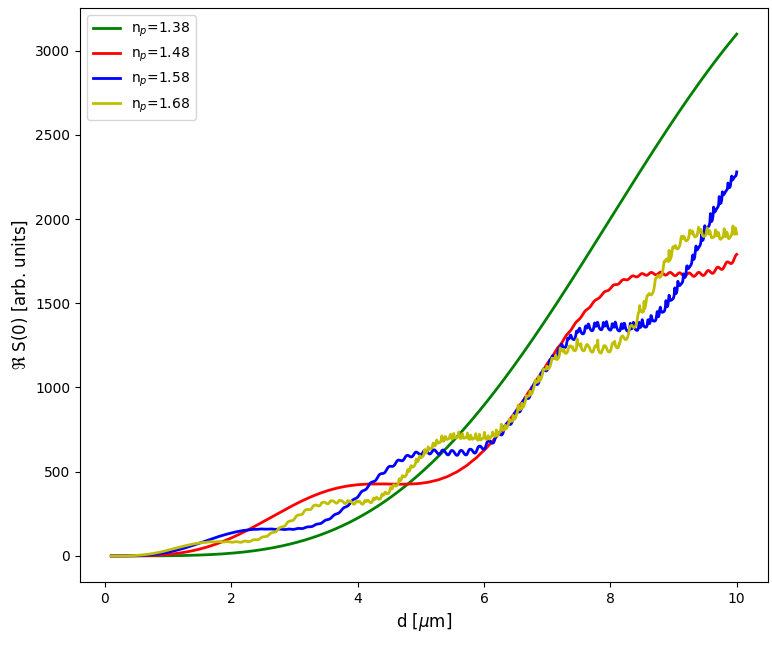
\includegraphics[scale=0.37]{ReS0_example.png}
	\caption{(a)}
	\end{subfigure} 
	\begin{subfigure}{.5\textwidth}
	\centering
	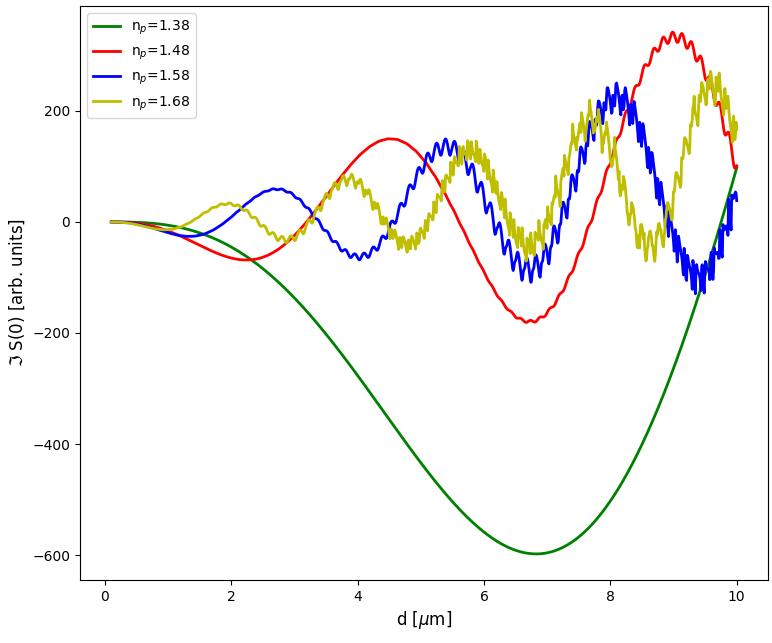
\includegraphics[scale=0.37]{ImS0_example.png}
	\caption{(b)}
	\end{subfigure} 
	\caption{Trend of $S\left( 0 \right)$ for an aqueous suspension spherical particles with different refractive indices, as a function of particles diameter between 0.1 and 10 $\mu$m.}
	\label{S0_example}
\end{figure}
\newline
Moreover, the real part of the complex scattering amplitude is directly linked to the extinction properties of the particle itself: we can define the extinction cross section as \cite{BH, VdH}	\begin{equation}
	C_{ext} = \dfrac{4\pi}{k^2}\Re\{ S(0) \}
	\label{cext_sphere}
\end{equation}
This is the fundamental extinction formula. The extinction process is not a blocking of the incoming wave but a subtle interference phenomenon where the scattered wave removes some of the energy of the original one by interference.
The forward scattered wave has an ever weaker influence with increasing $z$ extending over ever wider concentric circles in such a way that the total energy suppressed remains constant and equal to the energy incident on the area C$_{ext}$.
\newpage
In Fig.(\ref{cext_example}) are reported the extinction curves corresponding to the values of $\Re\{S(0)\}$ in Fig.(\ref{S0_example}a).
\begin{figure}[!htb]
	\centering	
	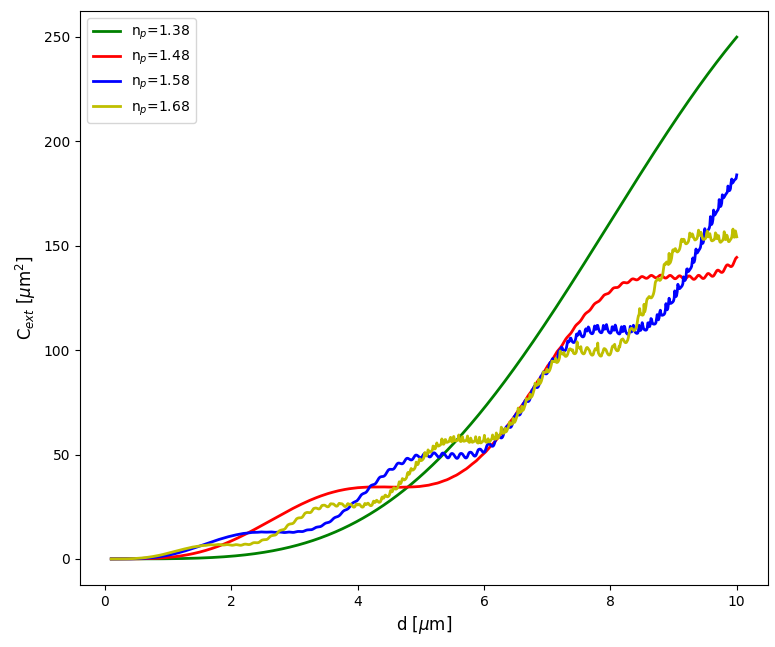
\includegraphics[scale=0.6]{Cext_example.png}
	\caption{Trend of C$_{ext}$ for an aqueous suspension spherical particles with different refractive indices, as a function of particles diameter between 0.1 and 10 $\mu$m.}
	\label{cext_example}
\end{figure}


%%%%%%%%%%%%%%%%%%%%%%%%%%%%%%%%%%%%%%%%%%%%%%%%%%%%%%%%%%%%%%%%%%%%%%%%%%%%%%%%%%%%
%%%%%%%%%%%%%%%%%%%%%%%%%%%%%%%%%%%%%%%%%%%%%%%%%%%%%%%%%%%%%%%%%%%%%%%%%%%%%%%%%%%%


\newpage
\chapter{Appendix B: software back-end examples and requirements}

\section{Folder organization}
The software folder is organized as reported in the following picture: 
\begin{figure}[!htb]
	\centering
	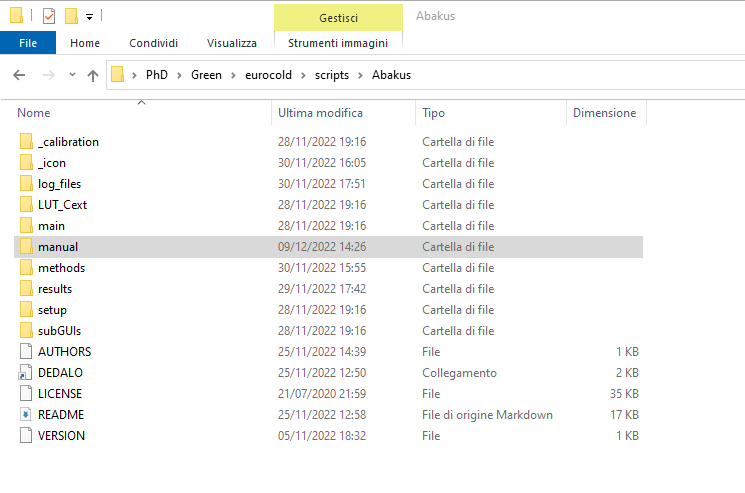
\includegraphics[scale=0.75]{folder.png}
	\caption{Abakus GUI software repository. The main script is the `abakus.pyw' (the first one), while the others are classes or supplementary modules useful for the software working correctly. Some subfolders are also listed containing text files and GUI configuration files.}
\end{figure}
\newline
In the following the different subfoolders are also presented.
\newpage
\begin{itemize}
\item the \textit{subGUIs} folder contains all the .ui files for defining the GUI layout;
\begin{figure}[!htb]
	\centering
	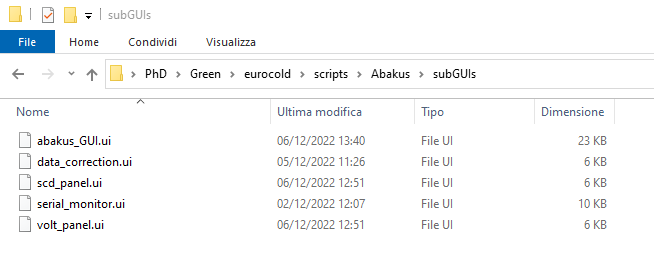
\includegraphics[scale=0.77]{folder_1.png}
\end{figure}
\item the \textit{methods} folder consists of some python scripts which perform different tasks;
\begin{figure}[!htb]
	\centering
	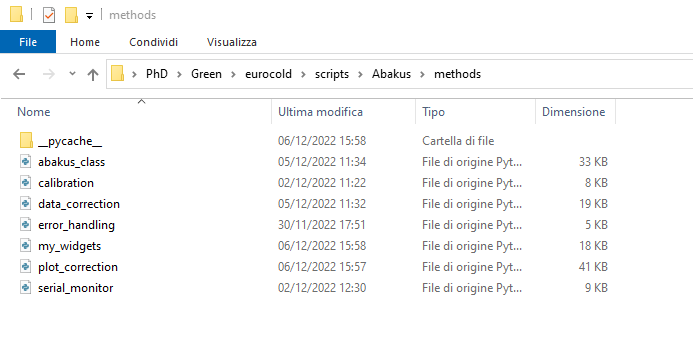
\includegraphics[scale=0.77]{folder_2.png}
\end{figure}
\item in the \textit{main} folder the main DEDALO script is located;
\item the \textit{setup} folder contains a text file and a setup.py script for installing all the required python packages;
\begin{figure}[!htb]
	\centering
	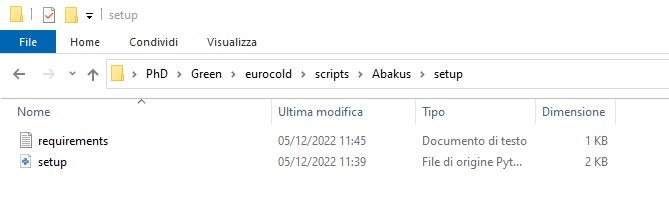
\includegraphics[scale=0.77]{folder_3.png}
\end{figure}
\newpage
\item in the \textit{LUT\textunderscore Cext} folder are stored some LUT (Look-Up Table) files for performing the data refractive index correction;
\begin{figure}[!htb]
	\centering
	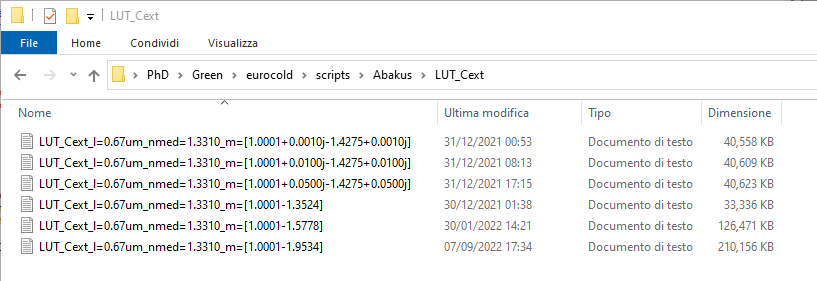
\includegraphics[scale=0.71]{folder_4.png}
\end{figure}
\item in the \textit{log\textunderscore files} folder a report file is saved every time some errors or warnings occur during the DEDALO running;
\begin{figure}[!htb]
	\centering
	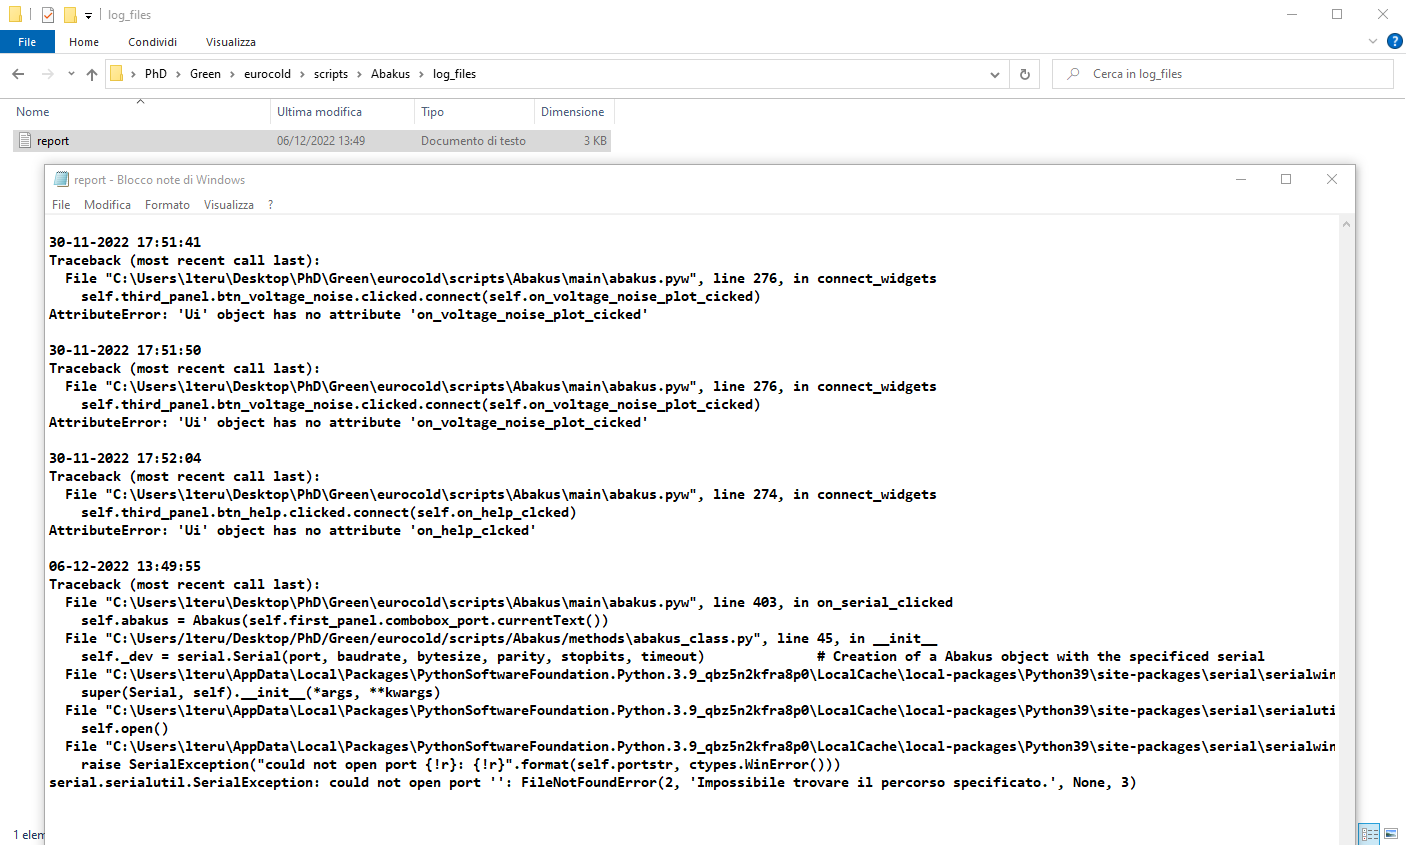
\includegraphics[scale=0.45]{folder_5.png}
\end{figure}
\item the \textit{manual} folder is the one where you are now;
\item the \textit{\textunderscore icon} folder contains all the icon and pictures that appears int eh GUI;
\item the \textit{\textunderscore calibration} folder stores two text files concerning the instrument calibration function;
\item in the \textit{results} folder, lastly, the output files of the DEDALO analyses are saved.
\end{itemize}

\section{Required packages and setup}
To run the script on his own laptop or PC, the user first need to install the specified Python packages:
\begin{itemize}
\item numpy $\geq$ 1.21, matplotlib $\geq$ 3.6.2 and math (default packages);
\item pyserial, for setting the serial communication through the RS232 port between the Abakus particle counter and the PC;
\item PyQt5, pyqtgraph, qtwidgets required for the graphical user interface;
\item termcolor;
\item pandas;
\item os-sys $\geq$ 2.1.4;
\item scipy $\geq$ 1.9.3 (optimize, interpolate), needed for computing the instrumental calibration curve;
\item miepython, for computations regardig Mie scattering parameters (eg. scattering and extinction cross sections);
\item openpyxl, for exporting data in xlsx files.
\end{itemize}
To do so, after installing Python3 and pip3, you can just copy and paste the following line in the command line: \\ \\
\texttt{pip3 install  numpy$\geq$1.21, matplotlib$\geq$3.6.2, os-sys$\geq$2.1.4, pyserial, PyQt5, \\ \hspace*{2.4 cm} pyqtgraph, qtwidgets, termcolor, scipy$\geq$1.9.3, miepython, openpyxl, \\ \hspace*{2.4 cm} pandas} \\ \\

Otherwise, you can run the setup.py script in the ''setup'' folder by typing: \\ \\
\texttt{python3 setup.py}

\newpage
\thispagestyle{plain}
\thispagestyle{empty}
\afterpage{\blankpage}


%%%%%%%%%%%%%%%%%%%%%%%%%%%%%%%%%%%%%%%%%%%%%%%%%%%%%%%%%%%%%%%%%%%%%%%%%%%%%%%%%%%%
%%%%%%%%%%%%%%%%%%%%%%%%%%%%%%%%%%%%%%%%%%%%%%%%%%%%%%%%%%%%%%%%%%%%%%%%%%%%%%%%%%%%


\addcontentsline{toc}{chapter}{Bibliografia}

\begin{thebibliography}{99}

\bibitem {CC} \url{http://stmichaelshospitalresearch.ca/wp-content/uploads/2015/09/Particle-Size-Analysis-Beckman-Coulter-Multisizer-4-Manual.pdf}

\bibitem {BH} C. F. Boren, D. R. Huffman, "Absorption and Light Scattering by Small Particles" (Wiley Science Paperback Series, New York, 1998).

\bibitem {scattering_sphere_1} S. Wolf, N.V. Voshchinnikov, "Mie scattering by ensembles of particles with very large size parameters", \textit{Computer Physics Communications}, \textbf{162}, 113-123 (2004).

\bibitem {VdH} H. C. van de Hulst, "Light Scattering by Small Particles" (Dover Publicaiton Inc., New York, 1981).

\end{thebibliography}

\newpage
\thispagestyle{plain}
\thispagestyle{empty}
\afterpage{\blankpage}


%%%%%%%%%%%%%%%%%%%%%%%%%%%%%%%%%%%%%%%%%%%%%%%%%%%%%%%%%%%%%%%%%%%%%%%%%%%%%%%%%%%%
%%%%%%%%%%%%%%%%%%%%%%%%%%%%%%%%%%%%%%%%%%%%%%%%%%%%%%%%%%%%%%%%%%%%%%%%%%%%%%%%%%%%


\end{document}
